\graphicspath{{LearningTetradPaper/LagrangianDeformationModels/figs/}}
% ------------------------------------------------------------------------%
\title{Velocity gradient prediction using parameterized Lagrangian deformation models}

\author{Criston Hyett, Yifeng Tian, Michael Woodward, Misha Stepanov,\\ Chris Fryer, Michael Chertkov, Daniel Livescu}


\begin{frame}
  \maketitle
\end{frame}
% ------------------------------------------------------------------------%

% ------------------------------------------------------------------------%
\begin{frame}{Motivation}
  \begin{itemize}
  \item The \textbf{velocity gradient tensor} (VGT) describes many important aspects of turbulence. It displays characteristic \textbf{non-Gaussian statistics} including \textbf{intermittency}, describes the \textbf{deformation of a fluid volume}, and encapsulates \textbf{alignment between strain and vorticity}.

  \item Similar to velocity in the Eularian frame, the VGT is the natural object of study in the \textbf{Lagrangian frame}.

  \item We combine \textbf{phenomenological models} of the VGT with \textbf{physics-informed machine learning} to create efficient (and interpretable?) \textbf{reduced-order models of the VGT}.
  \end{itemize}
  
\end{frame}
% ------------------------------------------------------------------------%

% ------------------------------------------------------------------------%
\begin{frame}{Governing Equations for the Velocity Gradient Tensor}
  \begin{itemize}
  \item The \textbf{velocity gradient tensor} (VGT) is defined by $A_{ij} = \frac{\partial u_i}{\partial x_j}$, so from Navier Stokes
    \begin{equation} \label{eq:NS}
      \frac{\partial u_i}{\partial t} + u_k \frac{\partial u_i}{\partial x_k} = -\frac{\partial P}{\partial x_i} + \nu \frac{\partial^2 u_i}{\partial x_k \partial x_k}
    \end{equation}

  \item We apply spatial derivatives, and use incompressibility to find the governing equations for the VGT:      
    \begin{equation}
      \frac{dA_{ij}}{dt} =
      - \colorboxed{green}{\left(A_{ik}A_{kj} + \frac{1}{3}A_{mn}A_{nm}\delta_{ij}\right)}
      - \colorboxed{red}{\left(\frac{\partial^2 P}{\partial x_i \partial x_j} -\frac{1}{3}\frac{\partial^2 P}{\partial x_k \partial x_k}\delta_{ij}\right)}
      + \colorboxed{blue}{\nu \frac{\partial^2 A_{ij}}{\partial x_k \partial x_k}}
    \end{equation}

  \item The main challenge is to predict the nonlocal \textbf{deviatoric} part of the pressure hessian, defined as
    \begin{equation}
      H_{ij} = - \left( \frac{\partial^2 P}{\partial x_i \partial x_j} - \frac{1}{3}\frac{\partial P}{\partial x_k \partial x_k}\delta_{ij}  \right)
    \end{equation}
  \end{itemize}
\end{frame}
% ------------------------------------------------------------------------%

% ------------------------------------------------------------------------%
\begin{frame}{Previous Work}
  \begin{columns}
    \column{0.4\textwidth}
    \begin{itemize}
    \item (a) Restricted Euler
    \item (b) Deviatoric Pressure Hessian
    \item (c) Viscous Term
    \item (d) Combined
    \end{itemize}

    \column{0.6\textwidth}
    \begin{figure}
      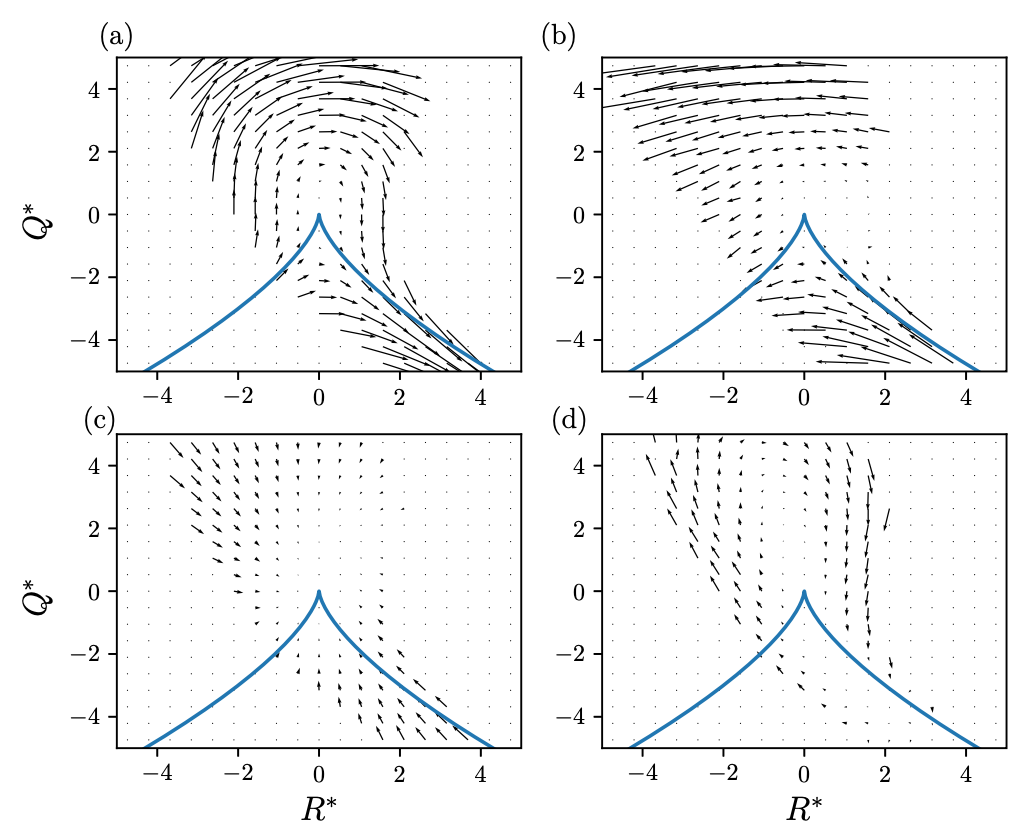
\includegraphics[width=\textwidth]{tian_qr_cmt.png}
      \caption{Figure taken from Tian et.al 2021}
    \end{figure}

  \end{columns}
\end{frame}
% ------------------------------------------------------------------------%

% ------------------------------------------------------------------------%
\begin{frame}{Tensor Basis Neural Network}
  \begin{itemize}
  \item We can write the formal solution for the deviatoric pressure hessian as\footcite{ohkitani1995}
    \begin{equation}
      H_{ij}(\textbf{x}) = \iiint \frac{\delta_{ij} - \hat{r_i}\hat{r_j}}{2\pi r^3}Q(\textbf{x} + \textbf{r})d\textbf{r}
    \end{equation}
  \item Using a Taylor expansion, Cayley-Hamilton Theorem, and Tensor Basis expansion\footcite{pope1975}, we can write
    \begin{equation}
      \hat{H} = \sum_{i=1}^{10} g^{(i)}(\lambda_1, \dots, \lambda_5)\cdot \hat{T}^{(i)}(\hat{A})
    \end{equation}
  \end{itemize}

  \begin{small}
    \begin{equation*}
      \lambda_1 = \tr(\hat{S}^2) \quad \lambda_2 = \tr(\hat{W}^2) \quad \lambda_3 = \tr(\hat{S}^3) \quad \lambda_4 = \tr(\hat{W}^2\hat{S}) \quad \lambda_5 = \tr(\hat{W}^2\hat{S}^2)
    \end{equation*}
  \end{small}

  \begin{itemize}
  \item We use the natural timescale $\tau = \langle \norm{S^2}_2 \rangle^{-1}$ to normalize our VGT, and thus all of the $\lambda_i, T^{(j)}$.
  \end{itemize}
\end{frame}
% ------------------------------------------------------------------------%

% ------------------------------------------------------------------------%
\begin{frame}{Tensor Basis Neural Network}

  \begin{equation}
    \hat{H} = \sum_{i=1}^{10} g\textcolor{blue}{_{\theta}}^{(i)}(\lambda_1, \dots, \lambda_5)\cdot \hat{T}^{(i)}(\hat{A})
  \end{equation}

  \begin{small}
    \begin{equation*}
      \lambda_1 = \tr(\hat{S}^2) \quad \lambda_2 = \tr(\hat{W}^2) \quad \lambda_3 = \tr(\hat{S}^3) \quad \lambda_4 = \tr(\hat{W}^2\hat{S}) \quad \lambda_5 = \tr(\hat{W}^2\hat{S}^2)
    \end{equation*}
  \end{small}
  \begin{figure}
    \centering
    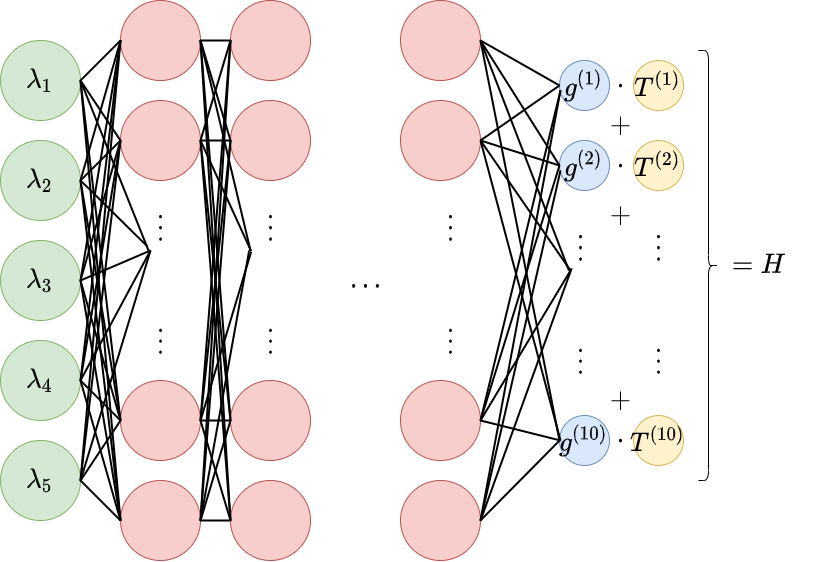
\includegraphics[width=0.5\textwidth]{./tbnn.png}
    \label{fig:tbnn}
  \end{figure}

  \begin{equation}
    L(\theta) = \frac{1}{N}\sum^N\norm{\hat{H}_{\text{truth}} - \sum_{i=1}^{10}g_\theta^{(i)}(\lambda_1, \dots, \lambda_5)T^{(i)}}_2^2
  \end{equation}
\end{frame}
% ------------------------------------------------------------------------%

% ------------------------------------------------------------------------%
\begin{frame}{Reproducing Results}
  \begin{figure}
    \centering
    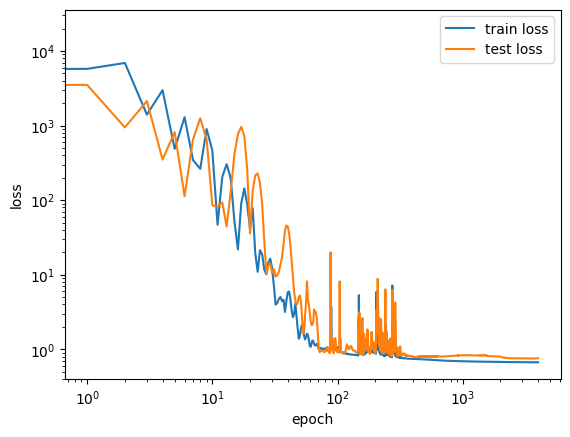
\includegraphics[width=0.5\textwidth]{trained_tbnn_loss.png}%
    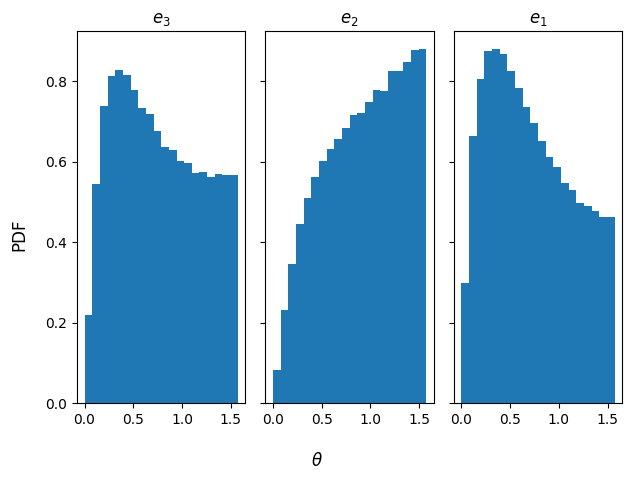
\includegraphics[width=0.4\textwidth]{tbnn_ph_eig_align.png}
    \caption{Implementing the architecture described, I show ability to train and reproduce loss plots (left) and eigenvector alignment PDFs (right)}
  \end{figure}
\end{frame}
% ------------------------------------------------------------------------%

% ------------------------------------------------------------------------%
\begin{frame}{Poking at Interpretability?}
  \begin{figure}
    \centering
    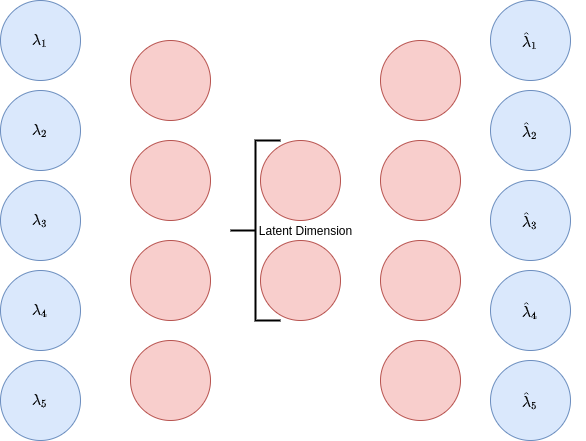
\includegraphics[width=0.5\textwidth]{aeStructure.png}%
    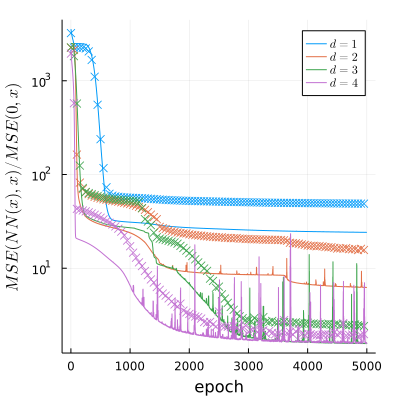
\includegraphics[width=0.5\textwidth]{aeInvariants.png}
  \end{figure}
\end{frame}
% ------------------------------------------------------------------------%

% ------------------------------------------------------------------------%
\begin{frame}{Poking at Interpretability?}
  \begin{figure}
    \centering
    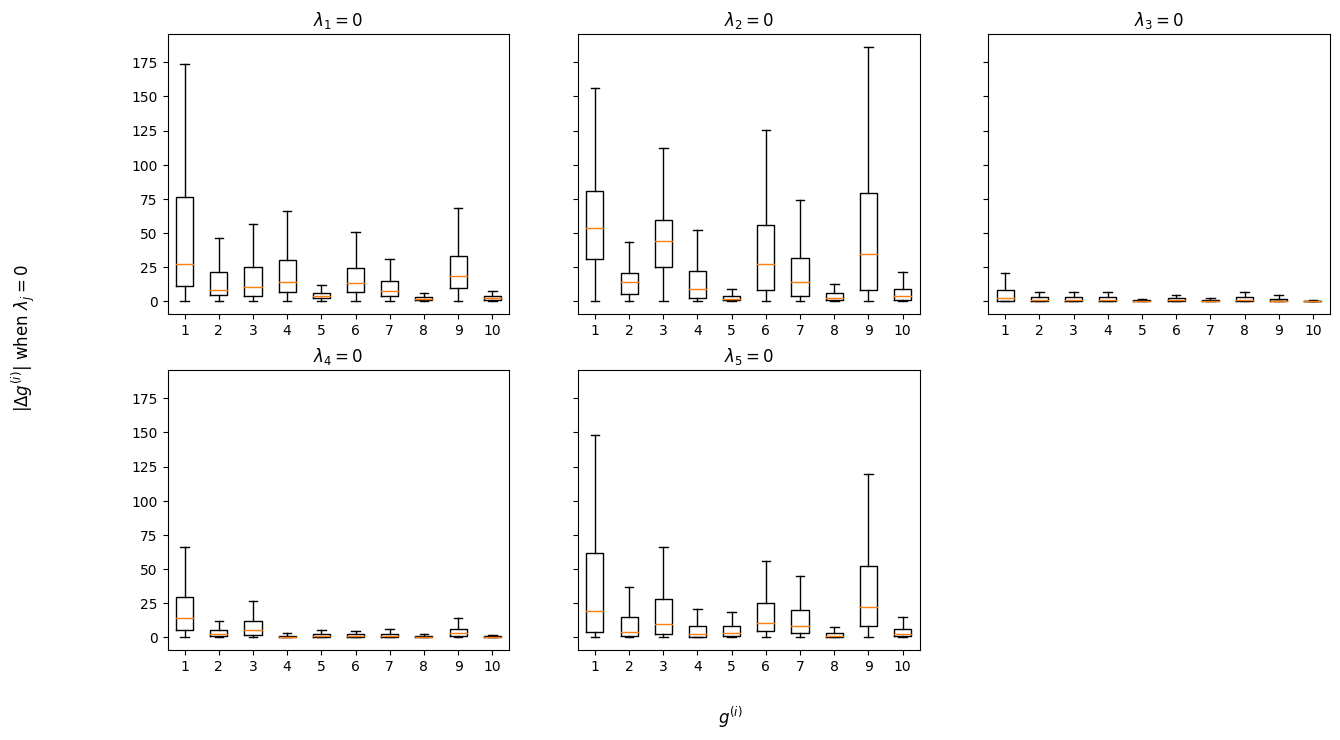
\includegraphics[width=\textwidth]{dg.png}
  \end{figure}
\end{frame}
% ------------------------------------------------------------------------%

% ------------------------------------------------------------------------%
\begin{frame}{Future Work}
  \begin{itemize}
  \item Work currently being done to enrich TBNN using history of the VGT
    \begin{itemize}
    \item Temporal convolutions? LSTM?
    \end{itemize}
  \item This work was originally inspired by the Tetrad model, and the coarse-grained velocity gradient tensor
    \begin{itemize}
    \item Particle-based coarse-graining and the opportunities/nuances/challenges is another challenge entirely
    \end{itemize}
  \item Can we learn physics?
    \begin{itemize}
    \item Interpretability
    \item Data-driven hypothesis testing
    \end{itemize}
  \end{itemize}
\end{frame}
% ------------------------------------------------------------------------%
